% Figure from MATH 591 notes, section 5. Compile with the notes preamble.
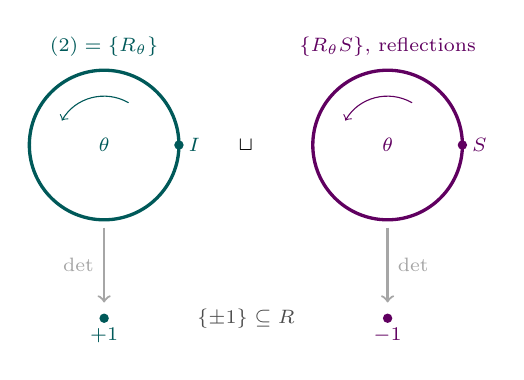
\begin{tikzpicture}
\draw[very thick, teal!70!black] (0.00,0) circle (0.95);
\fill[teal!70!black] (0.95,0) circle (1.7pt) node[anchor=west, font=\scriptsize] {$I$};
\node[teal!70!black, font=\scriptsize] at (0.00,1.25) {$\SO(2) = \{R_\theta\}$};
\draw[->, teal!70!black] (0.00,0) ++(60:0.62) arc (60:150:0.62); \node[font=\scriptsize, teal!70!black] at (0.00,0) {$\theta$};
\draw[very thick, violet!75!black] (3.60,0) circle (0.95);
\fill[violet!75!black] (4.55,0) circle (1.7pt) node[anchor=west, font=\scriptsize] {$S$};
\node[violet!75!black, font=\scriptsize] at (3.60,1.25) {$\{R_\theta S\}$, reflections};
\draw[->, violet!75!black] (3.60,0) ++(60:0.62) arc (60:150:0.62); \node[font=\scriptsize, violet!75!black] at (3.60,0) {$\theta$};
\node[font=\scriptsize, black!70] at (1.8,-2.2) {$\{\pm 1\} \subseteq \mathbb{R}$}; \fill[teal!70!black] (0,-2.2) circle (1.7pt) node[below, font=\scriptsize] {$+1$}; \fill[violet!75!black] (3.6,-2.2) circle (1.7pt) node[below, font=\scriptsize] {$-1$};
\draw[->, thick, gray!70] (0,-1.05) -- node[left, font=\scriptsize] {$\det$} (0,-2.0); \draw[->, thick, gray!70] (3.6,-1.05) -- node[right, font=\scriptsize] {$\det$} (3.6,-2.0);
\node[font=\scriptsize] at (1.8,0) {$\sqcup$};
\end{tikzpicture}
